% Options for packages loaded elsewhere
\PassOptionsToPackage{unicode}{hyperref}
\PassOptionsToPackage{hyphens}{url}
%
\documentclass[
]{book}
\usepackage{amsmath,amssymb}
\usepackage{iftex}
\ifPDFTeX
  \usepackage[T1]{fontenc}
  \usepackage[utf8]{inputenc}
  \usepackage{textcomp} % provide euro and other symbols
\else % if luatex or xetex
  \usepackage{unicode-math} % this also loads fontspec
  \defaultfontfeatures{Scale=MatchLowercase}
  \defaultfontfeatures[\rmfamily]{Ligatures=TeX,Scale=1}
\fi
\usepackage{lmodern}
\ifPDFTeX\else
  % xetex/luatex font selection
\fi
% Use upquote if available, for straight quotes in verbatim environments
\IfFileExists{upquote.sty}{\usepackage{upquote}}{}
\IfFileExists{microtype.sty}{% use microtype if available
  \usepackage[]{microtype}
  \UseMicrotypeSet[protrusion]{basicmath} % disable protrusion for tt fonts
}{}
\makeatletter
\@ifundefined{KOMAClassName}{% if non-KOMA class
  \IfFileExists{parskip.sty}{%
    \usepackage{parskip}
  }{% else
    \setlength{\parindent}{0pt}
    \setlength{\parskip}{6pt plus 2pt minus 1pt}}
}{% if KOMA class
  \KOMAoptions{parskip=half}}
\makeatother
\usepackage{xcolor}
\usepackage{color}
\usepackage{fancyvrb}
\newcommand{\VerbBar}{|}
\newcommand{\VERB}{\Verb[commandchars=\\\{\}]}
\DefineVerbatimEnvironment{Highlighting}{Verbatim}{commandchars=\\\{\}}
% Add ',fontsize=\small' for more characters per line
\usepackage{framed}
\definecolor{shadecolor}{RGB}{248,248,248}
\newenvironment{Shaded}{\begin{snugshade}}{\end{snugshade}}
\newcommand{\AlertTok}[1]{\textcolor[rgb]{0.94,0.16,0.16}{#1}}
\newcommand{\AnnotationTok}[1]{\textcolor[rgb]{0.56,0.35,0.01}{\textbf{\textit{#1}}}}
\newcommand{\AttributeTok}[1]{\textcolor[rgb]{0.13,0.29,0.53}{#1}}
\newcommand{\BaseNTok}[1]{\textcolor[rgb]{0.00,0.00,0.81}{#1}}
\newcommand{\BuiltInTok}[1]{#1}
\newcommand{\CharTok}[1]{\textcolor[rgb]{0.31,0.60,0.02}{#1}}
\newcommand{\CommentTok}[1]{\textcolor[rgb]{0.56,0.35,0.01}{\textit{#1}}}
\newcommand{\CommentVarTok}[1]{\textcolor[rgb]{0.56,0.35,0.01}{\textbf{\textit{#1}}}}
\newcommand{\ConstantTok}[1]{\textcolor[rgb]{0.56,0.35,0.01}{#1}}
\newcommand{\ControlFlowTok}[1]{\textcolor[rgb]{0.13,0.29,0.53}{\textbf{#1}}}
\newcommand{\DataTypeTok}[1]{\textcolor[rgb]{0.13,0.29,0.53}{#1}}
\newcommand{\DecValTok}[1]{\textcolor[rgb]{0.00,0.00,0.81}{#1}}
\newcommand{\DocumentationTok}[1]{\textcolor[rgb]{0.56,0.35,0.01}{\textbf{\textit{#1}}}}
\newcommand{\ErrorTok}[1]{\textcolor[rgb]{0.64,0.00,0.00}{\textbf{#1}}}
\newcommand{\ExtensionTok}[1]{#1}
\newcommand{\FloatTok}[1]{\textcolor[rgb]{0.00,0.00,0.81}{#1}}
\newcommand{\FunctionTok}[1]{\textcolor[rgb]{0.13,0.29,0.53}{\textbf{#1}}}
\newcommand{\ImportTok}[1]{#1}
\newcommand{\InformationTok}[1]{\textcolor[rgb]{0.56,0.35,0.01}{\textbf{\textit{#1}}}}
\newcommand{\KeywordTok}[1]{\textcolor[rgb]{0.13,0.29,0.53}{\textbf{#1}}}
\newcommand{\NormalTok}[1]{#1}
\newcommand{\OperatorTok}[1]{\textcolor[rgb]{0.81,0.36,0.00}{\textbf{#1}}}
\newcommand{\OtherTok}[1]{\textcolor[rgb]{0.56,0.35,0.01}{#1}}
\newcommand{\PreprocessorTok}[1]{\textcolor[rgb]{0.56,0.35,0.01}{\textit{#1}}}
\newcommand{\RegionMarkerTok}[1]{#1}
\newcommand{\SpecialCharTok}[1]{\textcolor[rgb]{0.81,0.36,0.00}{\textbf{#1}}}
\newcommand{\SpecialStringTok}[1]{\textcolor[rgb]{0.31,0.60,0.02}{#1}}
\newcommand{\StringTok}[1]{\textcolor[rgb]{0.31,0.60,0.02}{#1}}
\newcommand{\VariableTok}[1]{\textcolor[rgb]{0.00,0.00,0.00}{#1}}
\newcommand{\VerbatimStringTok}[1]{\textcolor[rgb]{0.31,0.60,0.02}{#1}}
\newcommand{\WarningTok}[1]{\textcolor[rgb]{0.56,0.35,0.01}{\textbf{\textit{#1}}}}
\usepackage{longtable,booktabs,array}
\usepackage{calc} % for calculating minipage widths
% Correct order of tables after \paragraph or \subparagraph
\usepackage{etoolbox}
\makeatletter
\patchcmd\longtable{\par}{\if@noskipsec\mbox{}\fi\par}{}{}
\makeatother
% Allow footnotes in longtable head/foot
\IfFileExists{footnotehyper.sty}{\usepackage{footnotehyper}}{\usepackage{footnote}}
\makesavenoteenv{longtable}
\usepackage{graphicx}
\makeatletter
\def\maxwidth{\ifdim\Gin@nat@width>\linewidth\linewidth\else\Gin@nat@width\fi}
\def\maxheight{\ifdim\Gin@nat@height>\textheight\textheight\else\Gin@nat@height\fi}
\makeatother
% Scale images if necessary, so that they will not overflow the page
% margins by default, and it is still possible to overwrite the defaults
% using explicit options in \includegraphics[width, height, ...]{}
\setkeys{Gin}{width=\maxwidth,height=\maxheight,keepaspectratio}
% Set default figure placement to htbp
\makeatletter
\def\fps@figure{htbp}
\makeatother
\setlength{\emergencystretch}{3em} % prevent overfull lines
\providecommand{\tightlist}{%
  \setlength{\itemsep}{0pt}\setlength{\parskip}{0pt}}
\setcounter{secnumdepth}{5}
\usepackage{booktabs}
\ifLuaTeX
  \usepackage{selnolig}  % disable illegal ligatures
\fi
\usepackage[]{natbib}
\bibliographystyle{plainnat}
\IfFileExists{bookmark.sty}{\usepackage{bookmark}}{\usepackage{hyperref}}
\IfFileExists{xurl.sty}{\usepackage{xurl}}{} % add URL line breaks if available
\urlstyle{same}
\hypersetup{
  pdftitle={現代人間論系演習(心を調べる・心理学実験)},
  pdfauthor={下司 忠大},
  hidelinks,
  pdfcreator={LaTeX via pandoc}}

\title{現代人間論系演習(心を調べる・心理学実験)}
\author{下司 忠大}
\date{最終更新日 2024-04-15}

\usepackage{amsthm}
\newtheorem{theorem}{Theorem}[chapter]
\newtheorem{lemma}{Lemma}[chapter]
\newtheorem{corollary}{Corollary}[chapter]
\newtheorem{proposition}{Proposition}[chapter]
\newtheorem{conjecture}{Conjecture}[chapter]
\theoremstyle{definition}
\newtheorem{definition}{Definition}[chapter]
\theoremstyle{definition}
\newtheorem{example}{Example}[chapter]
\theoremstyle{definition}
\newtheorem{exercise}{Exercise}[chapter]
\theoremstyle{definition}
\newtheorem{hypothesis}{Hypothesis}[chapter]
\theoremstyle{remark}
\newtheorem*{remark}{Remark}
\newtheorem*{solution}{Solution}
\begin{document}
\maketitle

{
\setcounter{tocdepth}{1}
\tableofcontents
}
\hypertarget{ux30a4ux30f3ux30c8ux30edux30c0ux30afux30b7ux30e7ux30f3}{%
\chapter*{イントロダクション}\label{ux30a4ux30f3ux30c8ux30edux30c0ux30afux30b7ux30e7ux30f3}}
\addcontentsline{toc}{chapter}{イントロダクション}

\hypertarget{ux62c5ux5f53ux6559ux54e1}{%
\subsection*{担当教員}\label{ux62c5ux5f53ux6559ux54e1}}
\addcontentsline{toc}{subsection}{担当教員}

下司 忠大(しもつかさ ただひろ)です。普段は立正大学の対人・社会心理学科で講師として研究をしています。早稲田大学大学院の文学研究科心理学コースで小塩真司先生のもとで博士号を取得し,2年間この早稲田大学の文学学術院で助手・助教として働いたあとに立正大学に着任しました。専門はパーソナリティ心理学で,ダーク・パーソナリティに関する研究をしてきました。

\hypertarget{ux672cux6f14ux7fd2ux306eux76eeux7684}{%
\subsection*{本演習の目的}\label{ux672cux6f14ux7fd2ux306eux76eeux7684}}
\addcontentsline{toc}{subsection}{本演習の目的}

本演習では,心理学的な仮説(例えば,実験群と統制群で記憶課題の成績に差があるかどうか,外向性とポジティブな感情との間には相関関係があるのだろうか,など)を検討するための様々な統計手法を演習形式で実践し,1.分析の実行,2.結果の読み取り,3.結果の記述ができることを目的とします。

\begin{itemize}
\tightlist
\item
  \href{https://www.dropbox.com/scl/fi/lu04wj6y6mjsht88sg20g/.pdf?rlkey=ng2r14napi2n2tz4wedm1eum7\&dl=0}{シラバス}
\end{itemize}

\hypertarget{ux6559ux79d1ux66f8ux306bux3064ux3044ux3066}{%
\subsection*{教科書について}\label{ux6559ux79d1ux66f8ux306bux3064ux3044ux3066}}
\addcontentsline{toc}{subsection}{教科書について}

本演習では教科書(小宮 あすか,布井 雅人 (著) 『\href{https://www.kspub.co.jp/book/detail/1548121.html}{Excelで今すぐはじめる心理統計 簡単ツールHADで基本を身につける}』講談社)に沿って授業を進めていきます。もし準備ができていない場合は必ず用意するようにしてください。

\hypertarget{ux6210ux7e3eux8a55ux4fa1ux306bux3064ux3044ux3066}{%
\subsection*{成績評価について}\label{ux6210ux7e3eux8a55ux4fa1ux306bux3064ux3044ux3066}}
\addcontentsline{toc}{subsection}{成績評価について}

平常点30\%(演習及び課題への取り組み姿勢),試験70\%(筆記試験: 15週目の定期試験日に実施)で評価します。試験は分析結果の読み取りに関するものです。

\hypertarget{ux6559ux54e1ux3068ux306eux30b3ux30f3ux30bfux30afux30c8}{%
\subsection*{教員とのコンタクト}\label{ux6559ux54e1ux3068ux306eux30b3ux30f3ux30bfux30afux30c8}}
\addcontentsline{toc}{subsection}{教員とのコンタクト}

私に何か連絡したいときは,Waseda Moodleのメッセージ機能(Messeage My Teacher)を利用してください。

\hypertarget{ux30c7ux30fcux30bfux5206ux6790ux306eux57faux790eux3068ux7d71ux8a08ux30bdux30d5ux30c8ux306eux64cdux4f5c}{%
\chapter{データ分析の基礎と統計ソフトの操作}\label{ux30c7ux30fcux30bfux5206ux6790ux306eux57faux790eux3068ux7d71ux8a08ux30bdux30d5ux30c8ux306eux64cdux4f5c}}

\hypertarget{ux76eeux7684}{%
\section{目的}\label{ux76eeux7684}}

今回の目的はデータ分析の基礎(尺度水準,記述統計・推測統計,統計的仮説検定)を理解するとともに,統計ソフトウェアHADを導入できるようになることです。今回の講義を通して,次回以降の実際のデータ分析のための土台を整えていきます。

\hypertarget{hadux306eux6e96ux5099}{%
\section{HADの準備}\label{hadux306eux6e96ux5099}}

\begin{itemize}
\tightlist
\item
  統計ソフトウェアHADをダウンロードしてみましょう。\\
\item
  教科書のp.1を開いてください。
\end{itemize}

\textbf{注意:教科書のp.2からのダウンロード方法はHADがOpen Science Framework (OSF) と呼ばれる研究者向けのツールサイトに保存されていた時代のものです。現在はHADはOne Driveに保存されているので,教科書とはダウンロード方法が異なります。}

\begin{itemize}
\tightlist
\item
  教科書のStep2までは同じ手順です。
\item
  「HADのダウンロード」をクリックすると,図1の画面が表示されます。
\end{itemize}

\begin{figure}
\centering
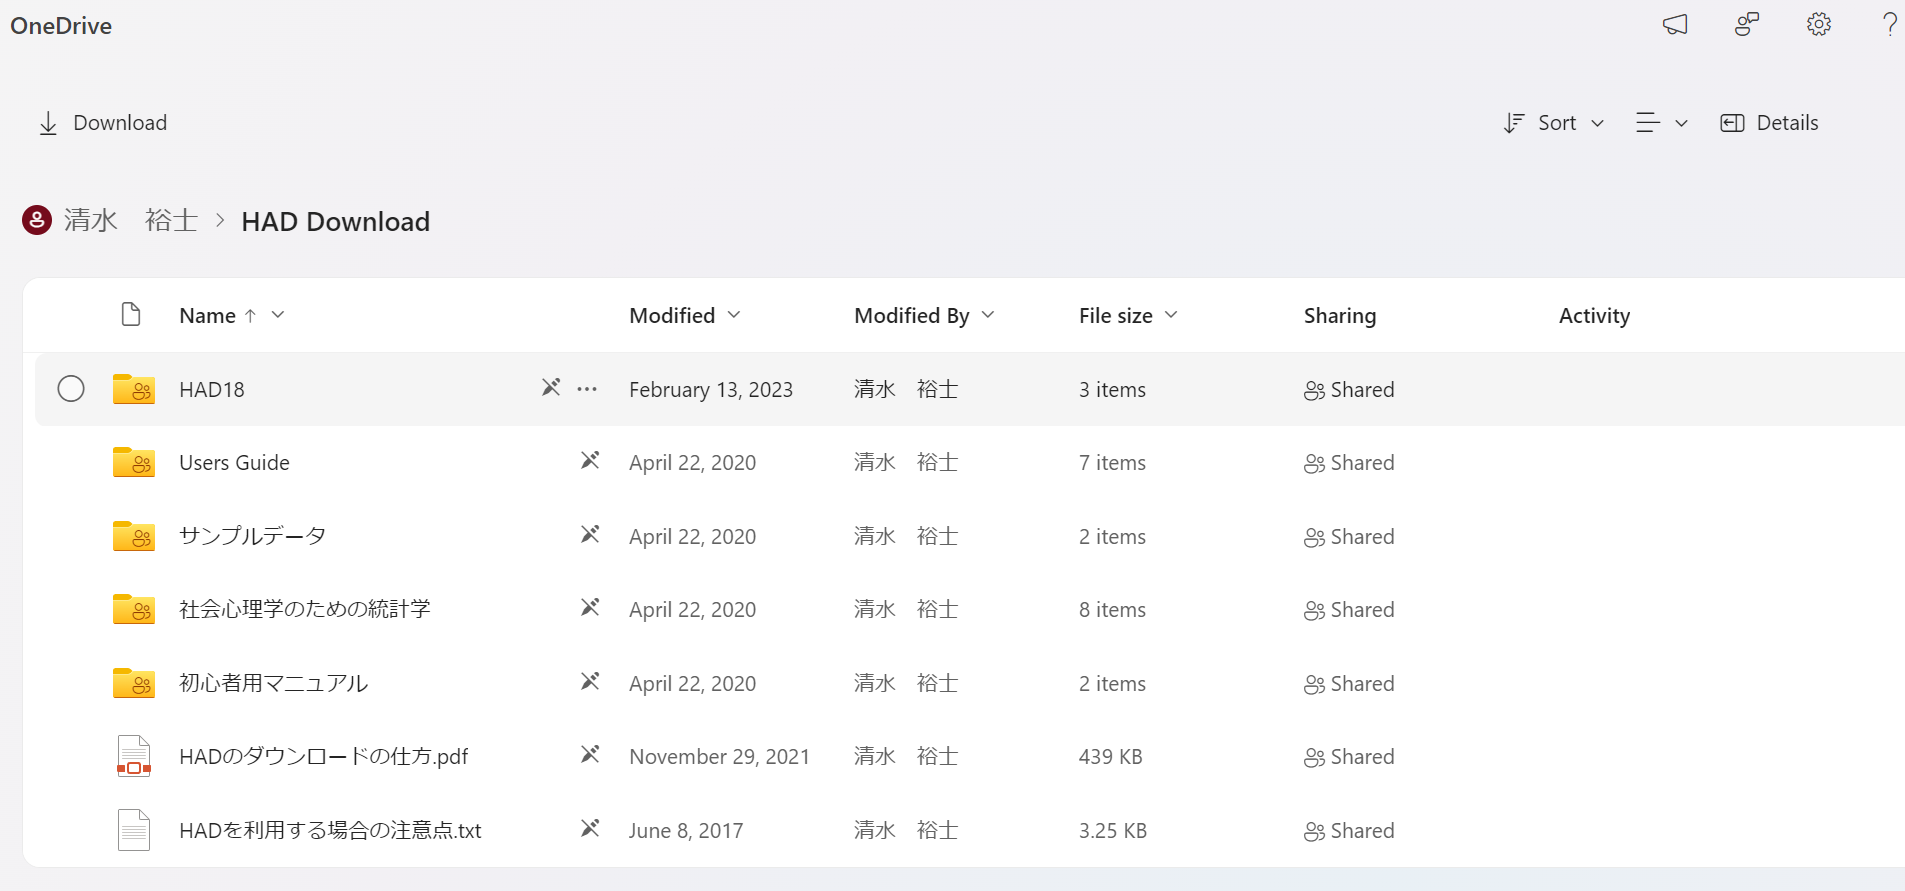
\includegraphics{images/1.1_HADのダウンロード1.png}
\caption{図1. HADのダウンロード画面1}
\end{figure}

\begin{itemize}
\tightlist
\item
  「HAD18」をクリックすると,図2の画面が表示されます。
\end{itemize}

\begin{figure}
\centering
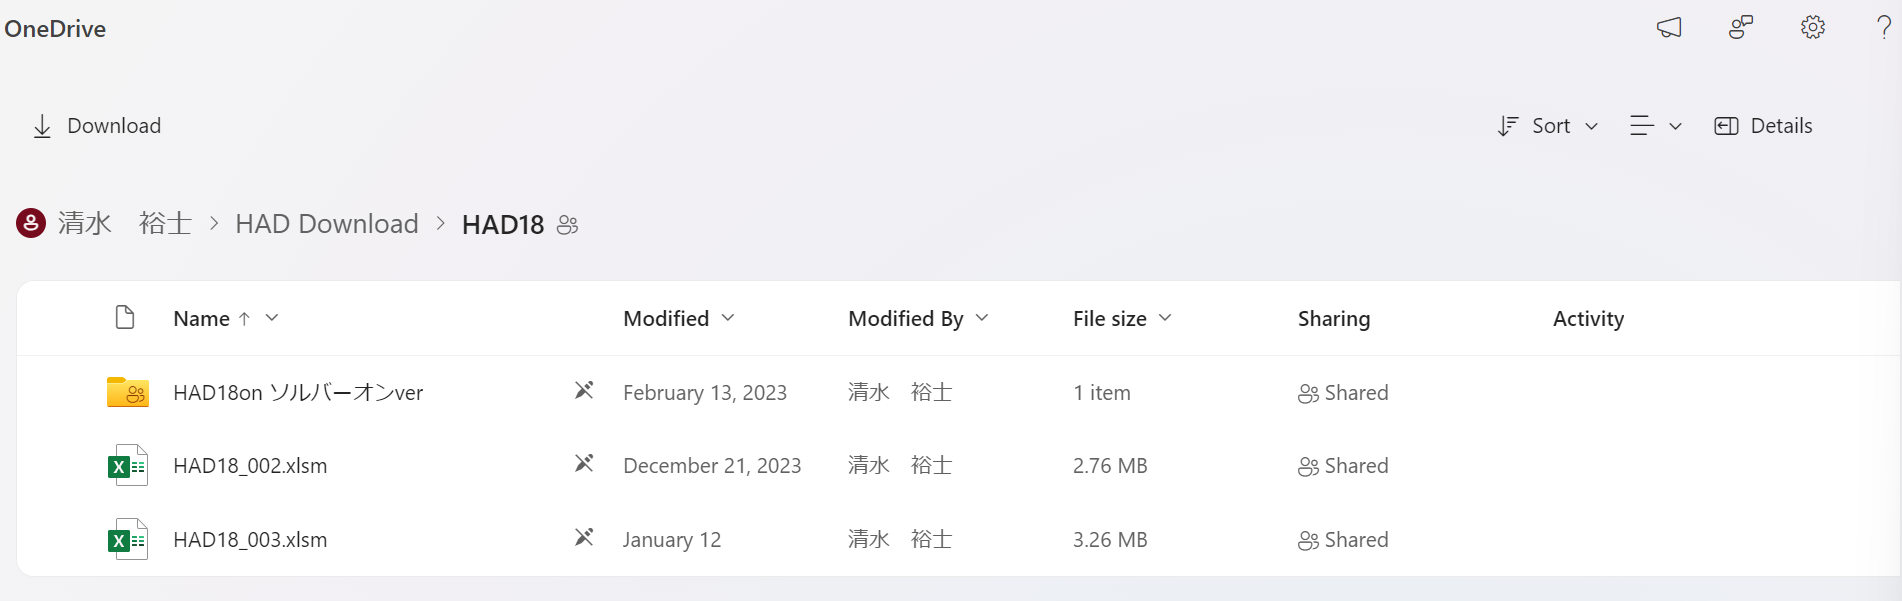
\includegraphics{images/1.1_HADのダウンロード2.png}
\caption{図2. HADのダウンロード画面2}
\end{figure}

\begin{itemize}
\tightlist
\item
  HADのバージョンについては教科書p.4のStep 5を参照してください。
\item
  ここでは,最新の「HAD18\_003.xlsm」をダウンロードしましょう。
\item
  「HAD18\_003.xlsm」にカーソルを合わせ「・・・」から「ダウンロード」を押してください。
\end{itemize}

\hypertarget{hadux3092ux958bux304f}{%
\section{HADを開く}\label{hadux3092ux958bux304f}}

\begin{itemize}
\tightlist
\item
  ダウンロードされたHADのファイルを開いてください。
\item
  開けたら,教科書p.5からの手順に沿ってデータの準備をしましょう。
\item
  HADは頻繁にダウンロードすることがあるので,手順を覚えておきましょう。
\end{itemize}

\textbf{\emph{注意:}}HADのファイルを開くときにエラーが表示されることがあります。具体的には,以下のような画面が表示されます。

\begin{figure}
\centering
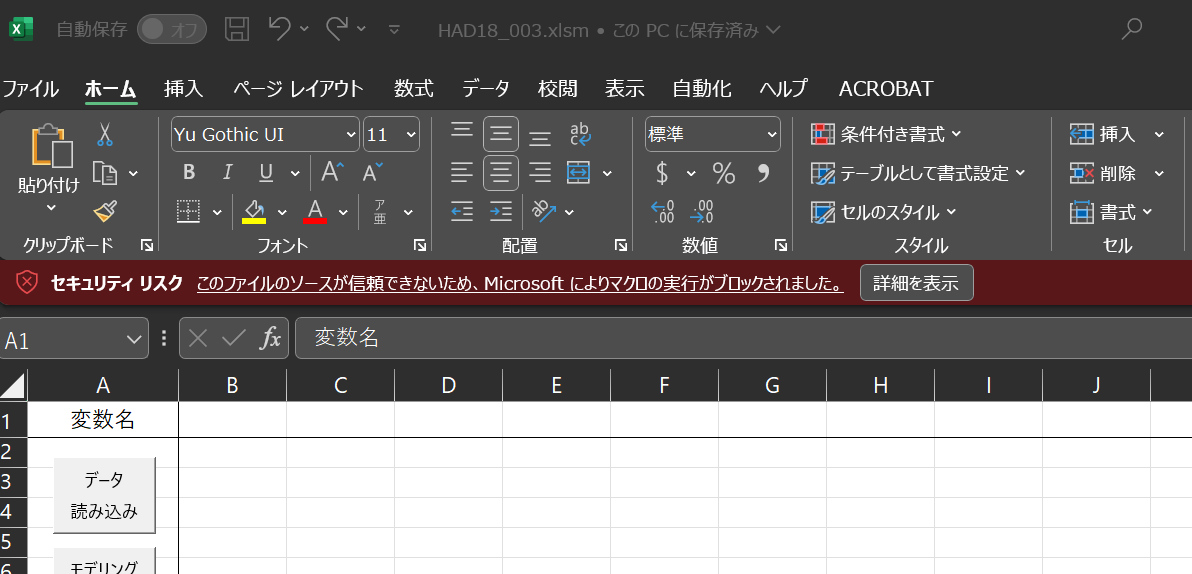
\includegraphics{images/1.2_HADのセキュリティエラー.png}
\caption{図3. HADのセキュリティエラー}
\end{figure}

この場合には,一度HADのファイルを閉じて,HADのファイルを右クリック→「プロパティ」を押し,「全般」→「セキュリティ」の「許可する」にチェックを入れて「OK」を押してください。この状態でもう一度HADのファイルを開くと,先ほどのエラーはなくなっているはずです。

\hypertarget{ux30c7ux30fcux30bfux5206ux6790ux306eux57faux790e}{%
\section{データ分析の基礎}\label{ux30c7ux30fcux30bfux5206ux6790ux306eux57faux790e}}

\begin{itemize}
\tightlist
\item
  そもそもなぜ心理学では統計を使うのか・心理統計の基礎知識を説明します。
\item
  教科書のp.7を開いてください。p.7-17(1-2章), p.39-47(4章)で説明します。
\end{itemize}

\hypertarget{ux7d71ux8a08ux7684ux4eeeux8aacux691cux5b9aux306bux3064ux3044ux3066}{%
\subsection{統計的仮説検定について}\label{ux7d71ux8a08ux7684ux4eeeux8aacux691cux5b9aux306bux3064ux3044ux3066}}

\begin{itemize}
\tightlist
\item
  統計的仮説検定の手続きの中では「検定統計量」が重要で,この値をもとに\emph{p}値が計算されます。
\item
  有意性検定を行う際には必ず検定統計量を使用するので,これから様々な分析を勉強するたびに,どのような検定統計量を使っているのかに注目してみてください。
\item
  また,p.45のチャートも,見通しを立てる上で有用です。
\item
  「平均値を比較するか」「2変数の関連を検討するか」という系統分けが大事なポイントで,実験法を用いる場合には平均値の比較,調査法を用いる場合には関連の検討が行われることが多いです。
\end{itemize}

\hypertarget{pux5024ux306bux3064ux3044ux3066}{%
\subsection{\texorpdfstring{\emph{p}値について}{p値について}}\label{pux5024ux306bux3064ux3044ux3066}}

\begin{itemize}
\tightlist
\item
  \emph{p}値は小さければ小さいほど帰無仮説を棄却しやすくなります。
\item
  \emph{p}値は効果が大きいほど小さくなりますが,サンプルサイズが多くても小さくなります。
\item
  つまり,\emph{p}値は必ずしも「効果の大きさ」を表すものではありません(教科書p.48 Tips参照)。
\item
  そのため,\emph{p}値とともに効果の大きさを直接表す「効果量」や「95\%信頼区間」を報告することがあります(効果量や95\%信頼区間については実際の分析の際に補足します)。
\end{itemize}

\hypertarget{ux8ad6ux6587ux3067ux5831ux544aux3059ux308bux5185ux5bb9ux306bux3064ux3044ux3066}{%
\subsection{論文で報告する内容について}\label{ux8ad6ux6587ux3067ux5831ux544aux3059ux308bux5185ux5bb9ux306bux3064ux3044ux3066}}

\begin{itemize}
\tightlist
\item
  教科書のp46-47に報告すべき心理統計用語がまとまっています。
\item
  本演習では報告すべき内容として,日本心理学会が発行する最新版の「\href{https://psych.or.jp/manual/}{執筆・投稿の手引き}」の結果セクションに従って進めていきます。
\end{itemize}

\hypertarget{ux30c7ux30fcux30bfux306eux6574ux7406ux8a18ux8ff0ux7d71ux8a08ux91cfux5ea6ux6570ux5206ux5e03ux8868}{%
\chapter{データの整理(記述統計量・度数分布表)}\label{ux30c7ux30fcux30bfux306eux6574ux7406ux8a18ux8ff0ux7d71ux8a08ux91cfux5ea6ux6570ux5206ux5e03ux8868}}

\hypertarget{ux76eeux7684-1}{%
\section{目的}\label{ux76eeux7684-1}}

今回の目的は統計ソフトHADでデータを読み込ませ,記述統計量やヒストグラム・度数分布表を算出し,その結果を報告できるようになることです。

\hypertarget{ux30b5ux30f3ux30d7ux30ebux30c7ux30fcux30bfux306eux8aadux307fux8fbcux307f}{%
\section{サンプルデータの読み込み}\label{ux30b5ux30f3ux30d7ux30ebux30c7ux30fcux30bfux306eux8aadux307fux8fbcux307f}}

\begin{itemize}
\tightlist
\item
  サンプルデータをダウンロードしてください。
\end{itemize}

\hypertarget{parts}{%
\chapter{Parts}\label{parts}}

You can add parts to organize one or more book chapters together. Parts can be inserted at the top of an .Rmd file, before the first-level chapter heading in that same file.

Add a numbered part: \texttt{\#\ (PART)\ Act\ one\ \{-\}} (followed by \texttt{\#\ A\ chapter})

Add an unnumbered part: \texttt{\#\ (PART\textbackslash{}*)\ Act\ one\ \{-\}} (followed by \texttt{\#\ A\ chapter})

Add an appendix as a special kind of un-numbered part: \texttt{\#\ (APPENDIX)\ Other\ stuff\ \{-\}} (followed by \texttt{\#\ A\ chapter}). Chapters in an appendix are prepended with letters instead of numbers.

\hypertarget{footnotes-and-citations}{%
\chapter{Footnotes and citations}\label{footnotes-and-citations}}

\hypertarget{footnotes}{%
\section{Footnotes}\label{footnotes}}

Footnotes are put inside the square brackets after a caret \texttt{\^{}{[}{]}}. Like this one \footnote{This is a footnote.}.

\hypertarget{citations}{%
\section{Citations}\label{citations}}

Reference items in your bibliography file(s) using \texttt{@key}.

For example, we are using the \textbf{bookdown} package \citep{R-bookdown} (check out the last code chunk in index.Rmd to see how this citation key was added) in this sample book, which was built on top of R Markdown and \textbf{knitr} \citep{xie2015} (this citation was added manually in an external file book.bib).
Note that the \texttt{.bib} files need to be listed in the index.Rmd with the YAML \texttt{bibliography} key.

The RStudio Visual Markdown Editor can also make it easier to insert citations: \url{https://rstudio.github.io/visual-markdown-editing/\#/citations}

\hypertarget{blocks}{%
\chapter{Blocks}\label{blocks}}

\hypertarget{equations}{%
\section{Equations}\label{equations}}

Here is an equation.

\begin{equation} 
  f\left(k\right) = \binom{n}{k} p^k\left(1-p\right)^{n-k}
  \label{eq:binom}
\end{equation}

You may refer to using \texttt{\textbackslash{}@ref(eq:binom)}, like see Equation \eqref{eq:binom}.

\hypertarget{theorems-and-proofs}{%
\section{Theorems and proofs}\label{theorems-and-proofs}}

Labeled theorems can be referenced in text using \texttt{\textbackslash{}@ref(thm:tri)}, for example, check out this smart theorem \ref{thm:tri}.

\begin{theorem}
\protect\hypertarget{thm:tri}{}\label{thm:tri}For a right triangle, if \(c\) denotes the \emph{length} of the hypotenuse
and \(a\) and \(b\) denote the lengths of the \textbf{other} two sides, we have
\[a^2 + b^2 = c^2\]
\end{theorem}

Read more here \url{https://bookdown.org/yihui/bookdown/markdown-extensions-by-bookdown.html}.

\hypertarget{callout-blocks}{%
\section{Callout blocks}\label{callout-blocks}}

The R Markdown Cookbook provides more help on how to use custom blocks to design your own callouts: \url{https://bookdown.org/yihui/rmarkdown-cookbook/custom-blocks.html}

\hypertarget{sharing-your-book}{%
\chapter{Sharing your book}\label{sharing-your-book}}

\hypertarget{publishing}{%
\section{Publishing}\label{publishing}}

HTML books can be published online, see: \url{https://bookdown.org/yihui/bookdown/publishing.html}

\hypertarget{pages}{%
\section{404 pages}\label{pages}}

By default, users will be directed to a 404 page if they try to access a webpage that cannot be found. If you'd like to customize your 404 page instead of using the default, you may add either a \texttt{\_404.Rmd} or \texttt{\_404.md} file to your project root and use code and/or Markdown syntax.

\hypertarget{metadata-for-sharing}{%
\section{Metadata for sharing}\label{metadata-for-sharing}}

Bookdown HTML books will provide HTML metadata for social sharing on platforms like Twitter, Facebook, and LinkedIn, using information you provide in the \texttt{index.Rmd} YAML. To setup, set the \texttt{url} for your book and the path to your \texttt{cover-image} file. Your book's \texttt{title} and \texttt{description} are also used.

This \texttt{gitbook} uses the same social sharing data across all chapters in your book- all links shared will look the same.

Specify your book's source repository on GitHub using the \texttt{edit} key under the configuration options in the \texttt{\_output.yml} file, which allows users to suggest an edit by linking to a chapter's source file.

Read more about the features of this output format here:

\url{https://pkgs.rstudio.com/bookdown/reference/gitbook.html}

Or use:

\begin{Shaded}
\begin{Highlighting}[]
\NormalTok{?bookdown}\SpecialCharTok{::}\NormalTok{gitbook}
\end{Highlighting}
\end{Shaded}


  \bibliography{book.bib,packages.bib}

\end{document}
